\documentclass{article}
\usepackage{enumitem}
\usepackage{pdfpages}
\usepackage{graphicx}
\begin{document}

\title{Homework \#1}
\author{Claire Trebing, Jason Young, Illya Starikov}
\date{Due Date: February 04, 2016}

\maketitle

\section*{Question 1}
\begin{enumerate}[label=\alph*]
\item Section's CRoom (Building and Room Number).
\item Section's DayTime and Year.
\item Section's SecID for every Year.
\end{enumerate}

\section*{Question 2}
\begin{center}
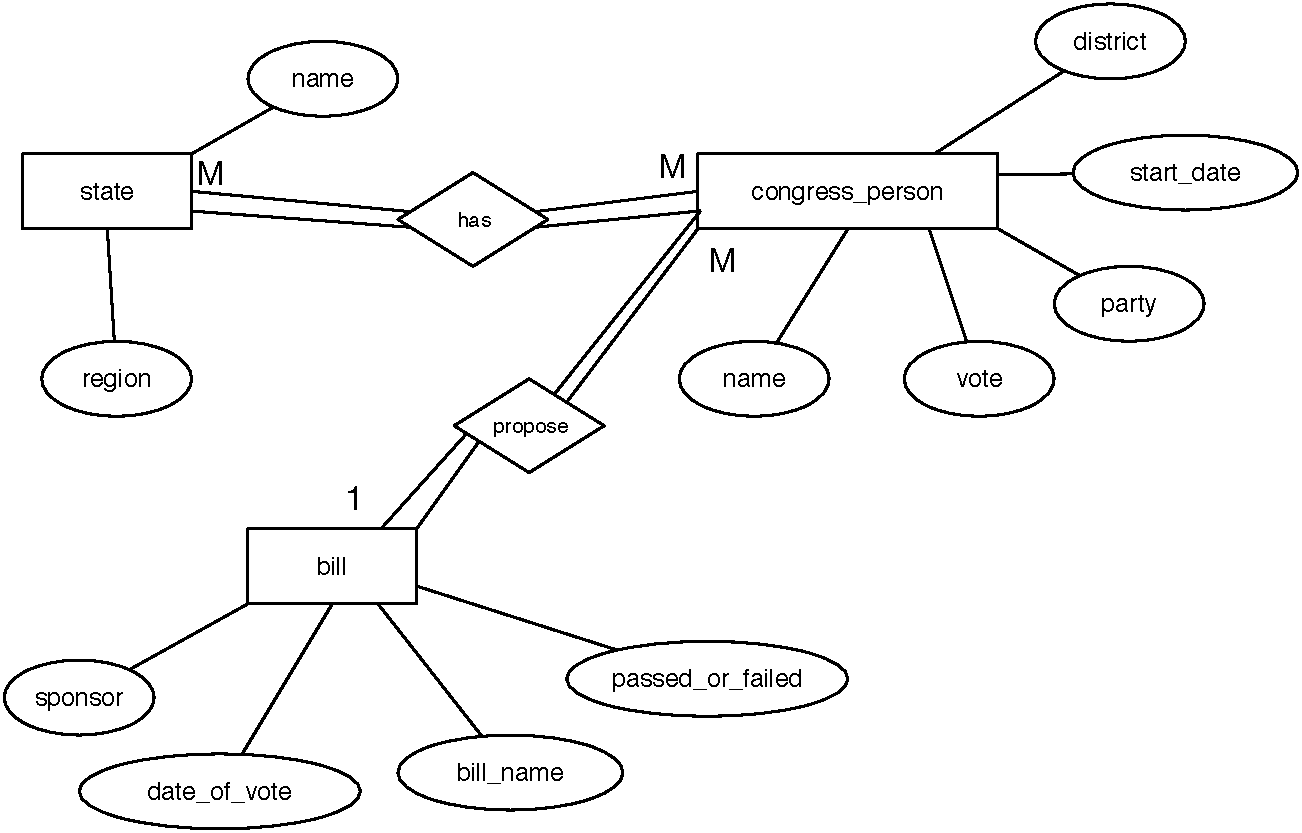
\includepdf[pages=-,width=1.25\textwidth]{2.pdf}
\end{center}


\section*{Question 3}
\begin{enumerate}[label=\alph*]
\item Strong Entity Types
    \begin{itemize}
    \item Bank
    \item Accounts
    \item Loans
    \item Customer
    \end{itemize}
\item Weak Entity Type
    \begin{itemize}
    \item Yes, the \textbf{Bank Branch} is a weak entity type. The partial key is the \textbf{Branch Number} and the identifying relationship is the \textbf{Branches} relationship.
    \end{itemize}
\item Constraints
    \begin{itemize}
    \item This information specifies that the branch number of a bank branch is only unique within a bank. For example, a bank branch in Bank A may have the same branch number as a bank branch in Bank B, but a bank branch in Bank A would not have the same branch number as any other bank branch in Bank A.
    \end{itemize}
\end{enumerate}

\section*{Question 4}
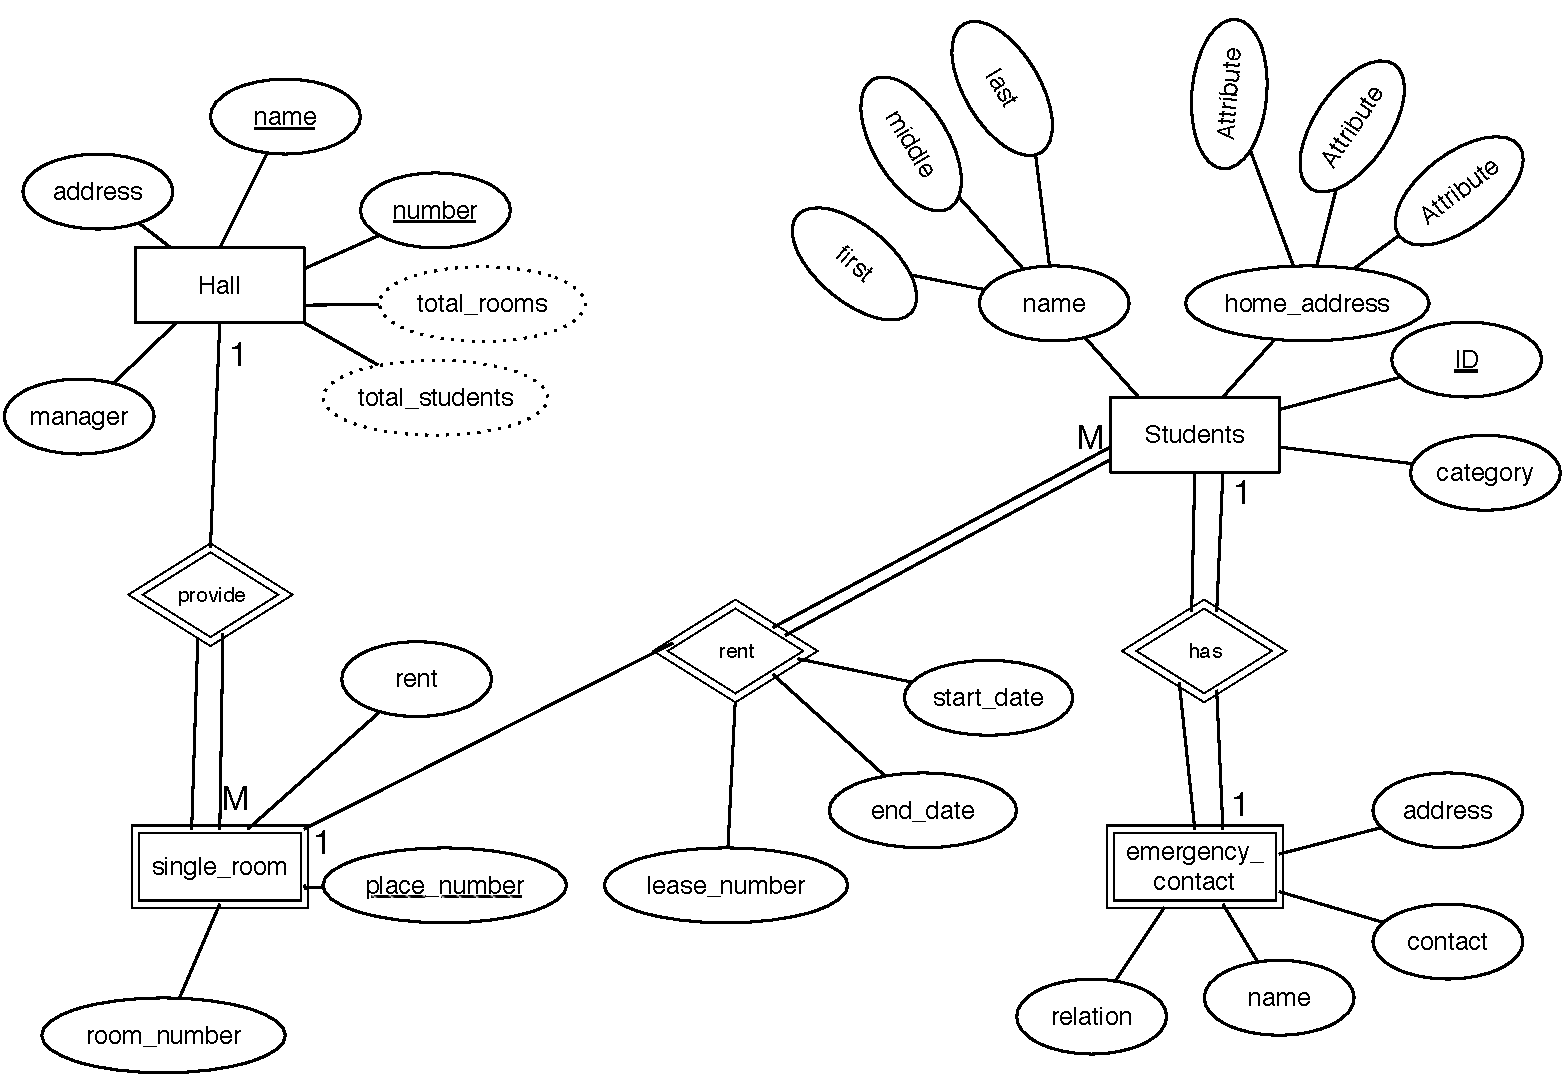
\includepdf[pages={1},width=1.25\textwidth]{4.pdf}

\end{document}